\chapter{رسم مدار با Fritzing}
هدف از این آزمایش بررسی اتصالات بردبورد و نحوه‌ی کار با آن است.
این نرم‌افزار تنها برای طراحی مدار است
 و فقط می‌توان با آن وصل بودن اتصالات را بررسی کرد.
 بنابراین قابلیت شبیه‌سازی در آن وجود ندارد.

 
\begin{figure}[h!]
\centering
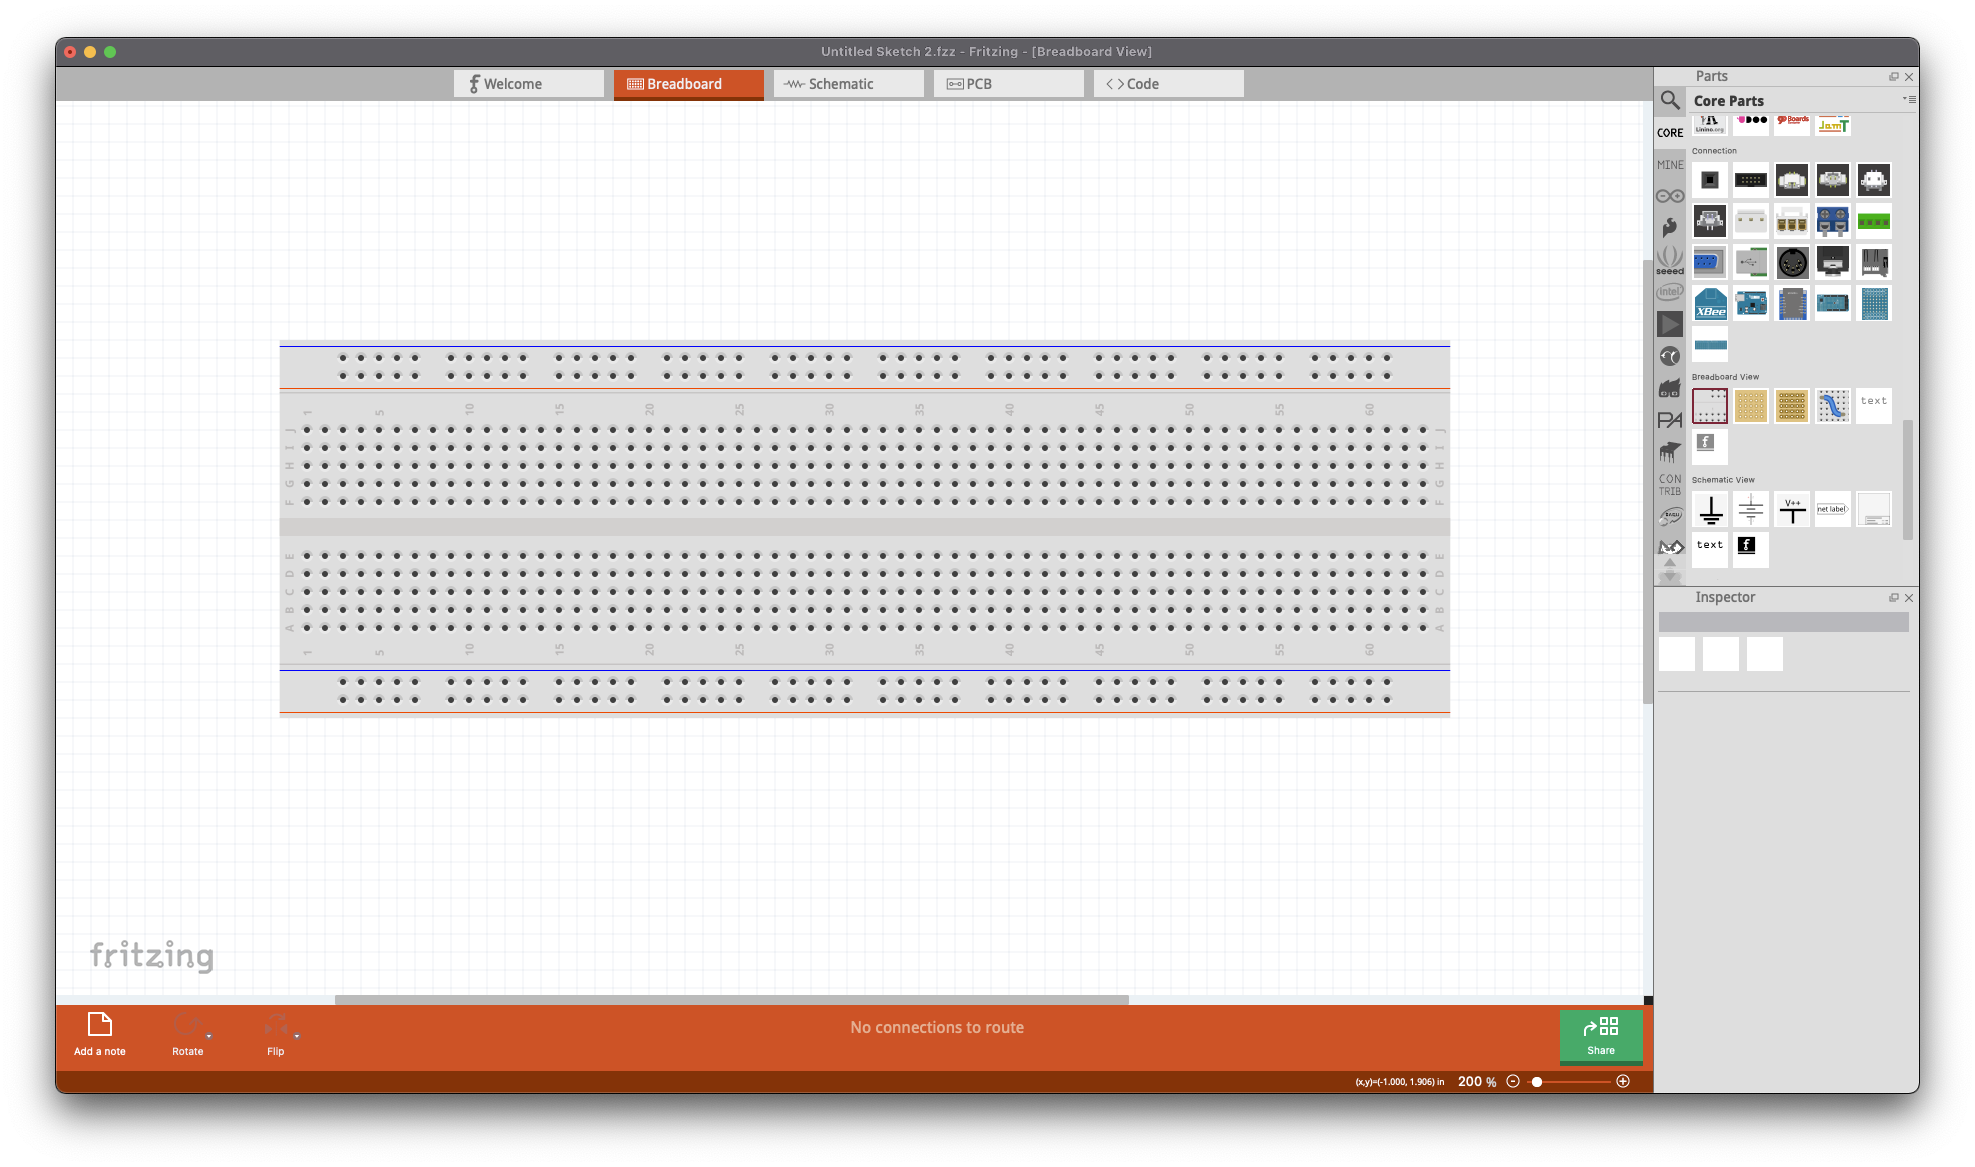
\includegraphics[scale=0.22]{introduction/1.png}    
\caption{محیط کار نرم‌افزار Fritzing}
\end{figure}
 
 
\section{اتصالات داخلی بردبورد}
در بالا و پایین برد بورد چهار نوار تغذیه وجود دارند که از هم مجزا هستند یعنی هیچ نواری
به نوار دیگر وصل نیست اما هر نوار در عرض کل برد بورد وصل است.
\begin{figure}[h!]
\centering
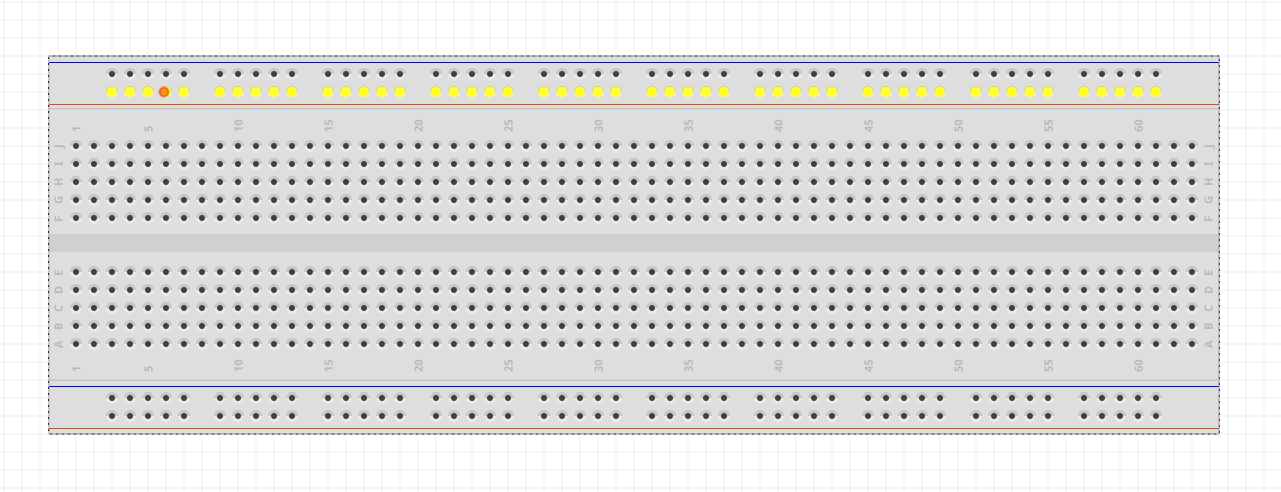
\includegraphics[scale=0.3]{introduction/3.png}    
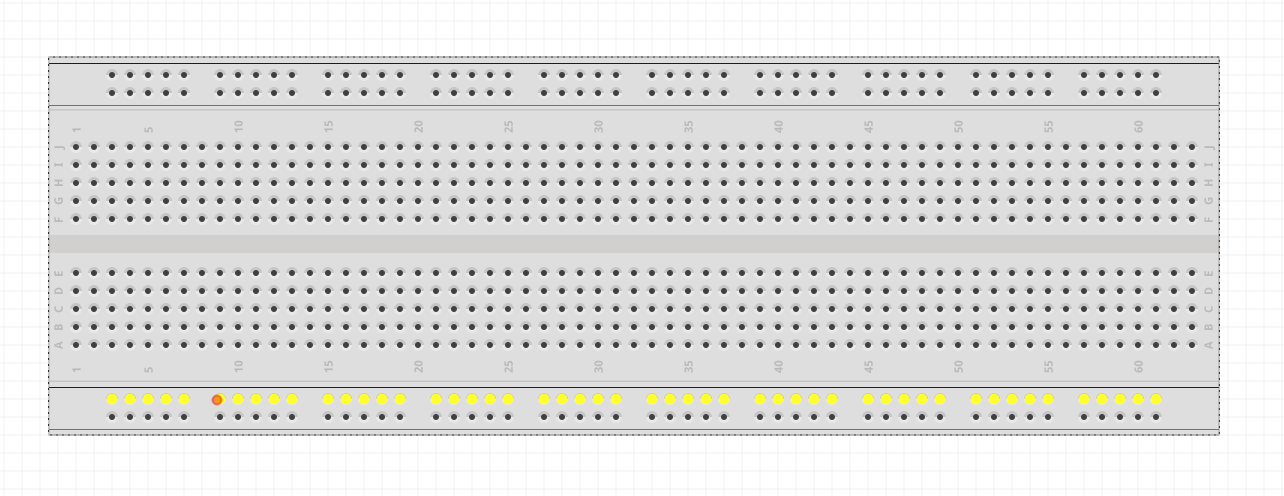
\includegraphics[scale=0.3]{introduction/4.png}    
\caption{دو تا از از نوارهای تغذیه بردبورد}
\end{figure}

در میانه‌ی برد بورد
ستون‌ها وجود دارند که هر ستون به اعضای خود وصل است.
اما ستون‌های بالا و پایین شکاف میانی به هم وصل نیستند.

\begin{figure}[h!]
\centering
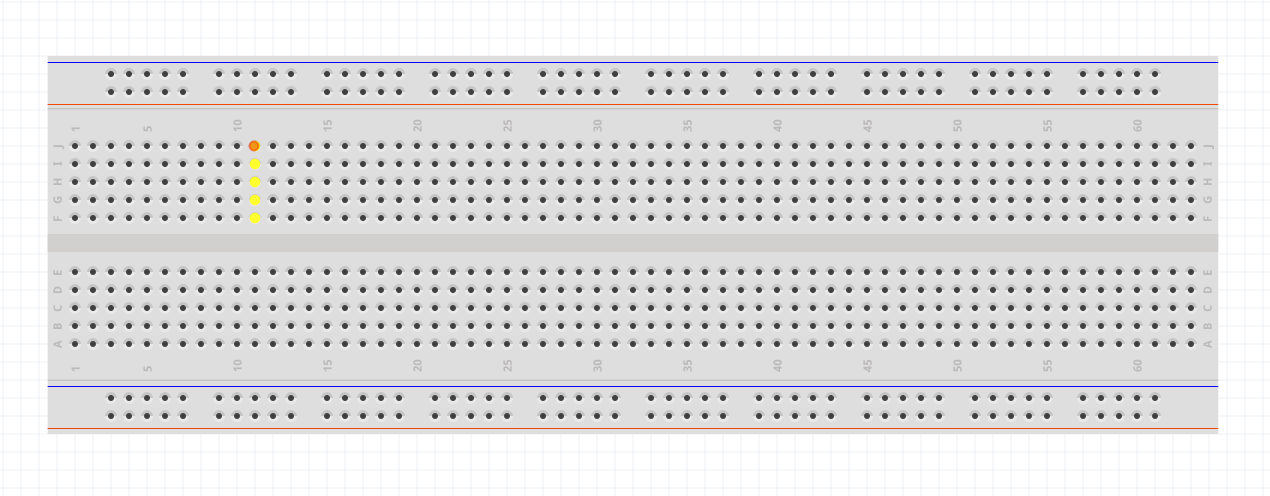
\includegraphics[scale=0.3]{introduction/2.png}    
\caption{یکی از ستون‌های اصلی}
\end{figure}

\section{
مدار LED
}
\subsection*{وسایل مورد نیاز}
\begin{enumerate}
    \item LED
    \item مقاومت 220 اهم
    \item منبع تغذیه 3 ولت
\end{enumerate}

\subsection*{تئوری آزمایش}
برای این آزمایش باید دقت کنیم پایه‌ّهای
LED
دارا جهت هستند و می‌بایست به مثبت و منفی بودن پایه‌ها دقت کرد.
برای تشخیص این امر به این نکته توجه می‌کنیم که داخل
LED
پایه‌ای که به تکه‌ی فلزی کوچک‌تر متصل است پایه‌ی مثبت است.
در صورتی که داخل LED
معلوم نبود به این نکته توجه داریم که معمولا پایه‌ی مثبت
LED
کمی بلند‌تر از پایه‌ی منفی است.

\begin{figure}[h!]
\centering
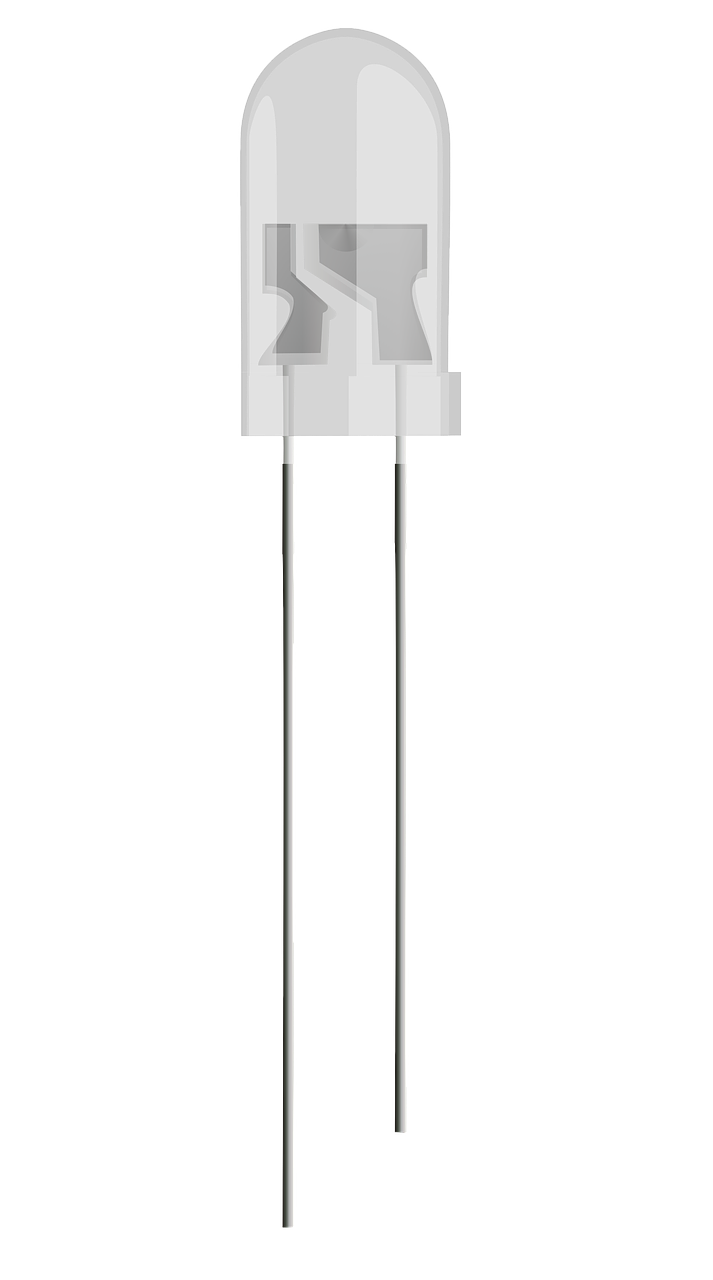
\includegraphics[scale=0.15]{introduction/led.png}    
\caption{یک LED معمولی}
\end{figure}

\subsection*{شرح آزمایش}
مطابق شکل مدار را به شکل صحیح بسته و به جهت پایه‌های
LED
توجه داریم.
همچنین برای تمیزی مدار باتری را به خطوط تغذیه بردبورد وصل می‌کنیم.
در ضمن اهمیتی ندارد مقاومت را در چه سمت
LED
قرار می‌دهیم زیرا در هر دو صورت معادله‌ی مدار یکسان است.


در انتها با قابلیت نرم‌افزار بررسی می‌کنیم تا اتصالات از ابتدای سر مثبت باتری تا جایی که
جریان به سر منفی می‌رسد برقرار باشد.

\begin{figure}[h]
\centering
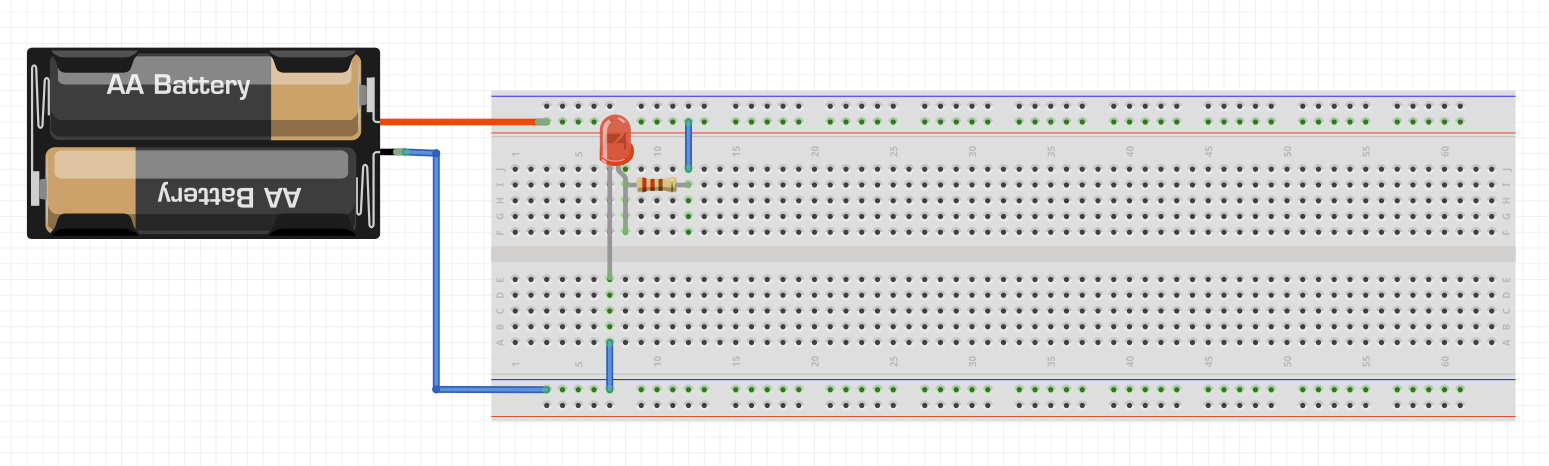
\includegraphics[scale=0.3]{introduction/5.png}    
\caption{مدار بخش ۲}
\end{figure}

\newpage
\section{نات نات نات نات نات نات}
\subsection*{وسایل مورد نیاز}
\begin{enumerate}
    \item LED
    \item 6 گیت نات
    \item منبع تغذیه 3 ولت
\end{enumerate}

\subsection*{تئوری آزمایش}
در نرم‌افزار به طور مستقیم قطعه‌ای با گیت نات وجود ندارد.
اما می‌دانیم با گیت
NOR
می‌توان گیت نات را ساخت.
برای این کار دو سر ورودی
NOR
را به هم وصل می‌کنیم.
با استفاده از دو آی‌سی
گیت
NOR
که هر کدام چهار گیت دارند، شش گیت نات مورد نیاز را خواهیم داشت.

\begin{figure}[h]
\centering
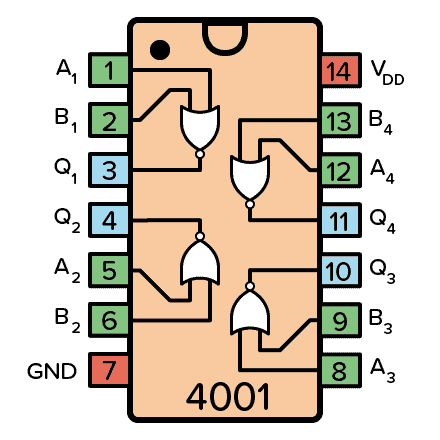
\includegraphics[scale=0.3]{introduction/not.png}    
\caption{مدار داخلی 4001}
\end{figure}

\subsection*{شرح آزمایش}
مطابق شکل ابتدا آی‌سی را روی شکاف بردبورد قرار داده و سپس تغذیه‌ی
آی‌سی‌ها را مطابق دیتاشیت‌شان
به آن‌ها وصل می‌کنیم.
معمولا پایه‌ی بالا سمت چپ VCC
و پایه‌ی پایین سمت راست
منفی یا زمین است.
دقت کنید که این بالا و پایین به شرطی است که نیم‌دایره‌ی فرورفته‌ی آی‌سی را در سمت چپ قرار دهیم و قطعه را نگاه کنیم.

حال که تغذیه‌ی آی‌سی‌ها وصل شد،
آن‌ها آماده‌ی کار هستند و آن‌ها را مطابق توضیحات بخش تئوری وصل می‌کنیم.


نکته‌ی مهم دیگر این که معمولا دیودهای نوری یا همان 
LED
برای ولتاژ حداکثر حدود
1.5 ولت طراحی شده‌اند.
که اینجا با اتصال باتری
3 
ولت بدون مقاومت ممکن است باعث سوختن LED
شویم.

همچنین بعضی از آی‌سی‌ها برای کار کردن به تغذیه‌ی بیشتر از 3 ولت
و در حدود 
5
ولت احتیاج دارند که اینجا فرض می‌کنیم هم LED و هم
آی‌سی با ولتاژ 3 ولت به درستی کار می‌کنند.


\begin{figure}[h]
\centering
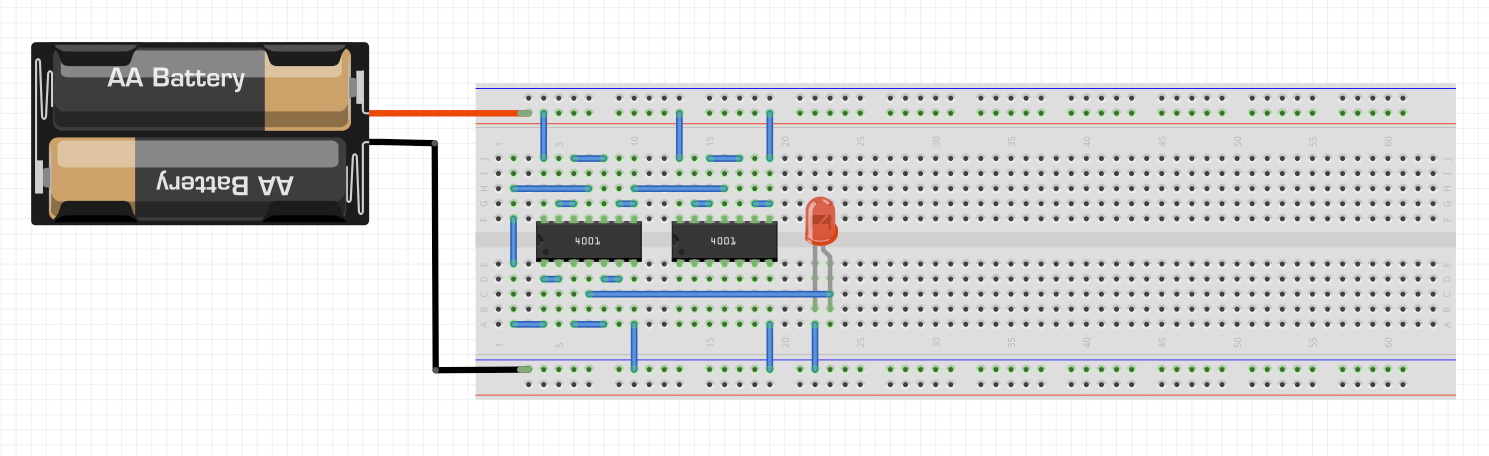
\includegraphics[scale=0.3]{introduction/6.png}    
\caption{مدار بخش 3}
\end{figure}